\documentclass[11pt]{article} 
\usepackage[letterpaper, margin=0.5in]{geometry}        		
\geometry{letterpaper}
\usepackage[parfill]{parskip} 
\usepackage{framed}
\usepackage{graphicx}
\usepackage{amsmath}
\usepackage{amssymb}
\usepackage{qtree}
\usepackage{makecell}
\usepackage{lmodern}
\renewcommand*\familydefault{\sfdefault}
\usepackage{tikz}
\usetikzlibrary{matrix}
\usepackage{tikz-qtree}

\usepackage{mathtools}
\DeclarePairedDelimiter\ceil{\lceil}{\rceil}
\DeclarePairedDelimiter\floor{\lfloor}{\rfloor}
\DeclarePairedDelimiter\abs{\lvert}{\rvert}%
\DeclarePairedDelimiter\norm{\lVert}{\rVert}%
    % \abs & \norm resizes brackets, starred version doesn't
    \makeatletter
    \let\oldabs\abs
    \def\abs{\@ifstar{\oldabs}{\oldabs*}}
    %
    \let\oldnorm\norm
    \def\norm{\@ifstar{\oldnorm}{\oldnorm*}}
    \makeatother

\newcommand\graytag[1]{\text{\textsl{\color{gray}{#1}}}}
\newcommand\tab[1][0.5cm]{\hspace*{#1}}
\newcommand\imp{\rightarrow}
\newcommand\thfr{\tab \therefore \tab}
\newcommand\sameas{\tab \equiv \tab}

\graphicspath{{../pdf/}{D:\Users\elizabethhoward\Documents\Courses\Current\csc263\assignments\a3}}

\title{CSC263 - Assignment 3}
\author{Cristyn Howard}
\date{Tuesday, Februrary 13, 2018}

\begin{document}
\maketitle

\subsection*{Question 1}	% 	My Answer to Question 1	%
\begin{center}
\begin{tabular}{lcl}

a) & & b) \\

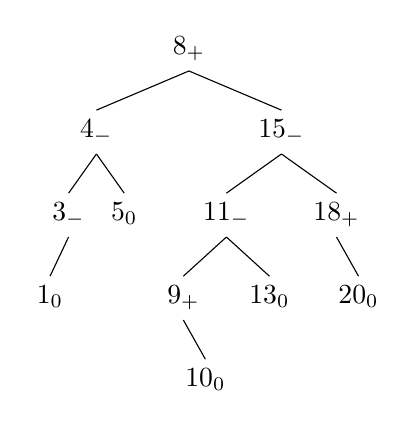
\begin{tikzpicture}     
\Tree [.$8_+$ 
        			[.$4_-$ 
            				[.$3_-$ 	
							\edge[]; {$1_0$}
                						\edge[draw=none]; {} ]
             				$5_0$ ] 
          		[.$15_-$	
					[.$11_-$	
							[.$9_+$	
									\edge[draw=none]; {}
									\edge[]; {$10_0$} ] 
							$13_0$ ]
					[.$18_+$	
							\edge[draw=none]; {}
							\edge[]; {$20_0$} ] ] ]
\end{tikzpicture}
& & 
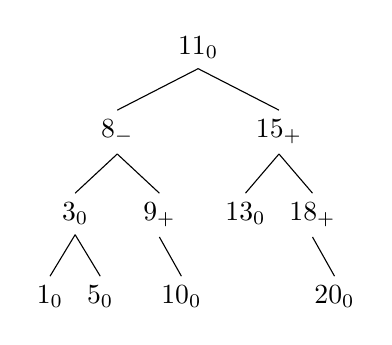
\begin{tikzpicture}     
\Tree [.$11_0$ 
        			[.$8_-$ 
            				[.$3_0$ 	
							$1_0$
                						$5_0$ ]
             				[.$9_+$ 
							\edge[draw=none]; {}
							\edge[]; {$10_0$} ] ] 
          		[.$15_+$	
					$13_0$
					[.$18_+$	
							\edge[draw=none]; {}
							\edge[]; {$20_0$} ] ] ]
\end{tikzpicture}

\end{tabular}
\end{center}
. \hrulefill

\subsection*{Question 2}	% 	My Answer to Question 2	 %
\begin{itemize}
\item[a)] Let each integer $i \in S$ serve as the key for a node in an AVL tree. 
\item[] Each node $x$ additionally stores:
	\begin{itemize}
	\item x.count $:$ number of nodes in the subtree rooted at x whose keys are less than or equal to x.key (x included) \\
	\tab[1.2cm] \graytag{$|R|, \text{  where  } \: [i \in R \subset S] \:\: \leftrightarrow \:\: [ (i \in x.subtree) \land (i.key \leq x.key) ]$ }
	\item x.keysum $:$ sum of keys of nodes in subtree rooted at x that are less than or equal to x.key (x included) \\
	\tab[1.2cm] \graytag{$\sum i.key \:\:\: \forall i \in x.subtree \subset S \:\: | \:\: i.key \leq x.key $ }
	\end{itemize}
\item[] Note that for a node $z$ with no children, we have z.count = 1 and z.keysum = z.key.
\item[] Here is an example, taken from question 1a: \\
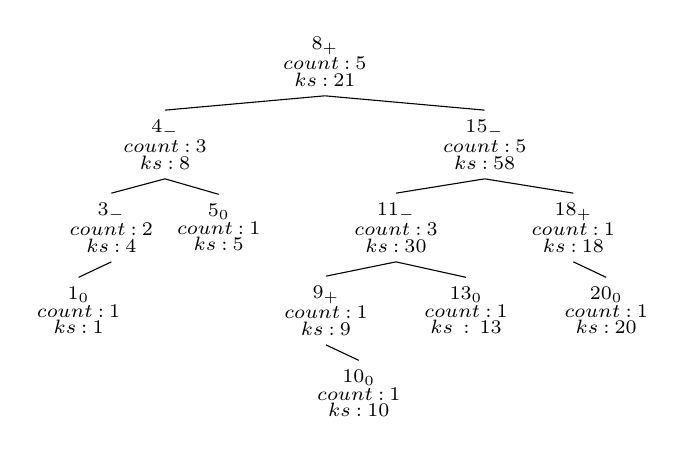
\begin{tikzpicture}     
\Tree [.$\substack{8_+ \\ count\::\:5 \\ ks\::\:21 }$
        			[.$\substack{4_- \\ count\::\:3 \\ ks\::\:8 }$ 
            				[.$\substack{3_- \\ count\::\:2\\ ks\::\:4}$ 	
							\edge[]; {$\substack{1_0 \\ count\::\:1\\ ks\::\:1}$}
                						\edge[draw=none]; {} ]
             				$\substack{5_0 \\ count\::\:1\\ ks\::\:5}$ ] 
          		[.$\substack{15_- \\ count\::\: 5 \\ ks\::\: 58}$	
					[.$\substack{11_- \\ count\::\:3 \\ ks\::\:30 }$	
							[.$\substack{9_+ \\ count\::\:1 \\ ks\::\:9 }$	
									\edge[draw=none]; {}
									\edge[]; {$\substack{10_0 \\ count\::\:1 \\ ks\::\:10 }$} ] 
							$\substack{13_0 \\ count\::\:1 \\ ks\:\::\:\:13 }$ ]
					[.$\substack{18_+ \\ count\::\:1 \\ ks\::\:18 }$	
							\edge[draw=none]; {}
							\edge[]; {$\substack{20_0 \\ count\::\:1 \\ ks\::\:20 }$} ] ] ]
\end{tikzpicture}
\newpage

\item [b)] ADD($i$)
	\begin{enumerate}
	\item create node $x$ with key $i$, then insert $x$ as in normal AVL tree (BST insert, rebalance)
		\begin{itemize}
		\item Whenever rebalancing means that a subtree $y.subtree$ (i.e. subtree rooted at y) becomes the new \textbf{left} child of node $z$, $z$ and all ancestor nodes of $z$ with keys is greater than or equal to $z.key$ must be amended so that: $zOrAncestorOfZ.keysum += y.keysum, zOrAncestorOfZ.count += y.count$
		\end{itemize}
	\item go up ancestor nodes of $x$ in it's final position until root is reached, and for each ancestor node whose key is greater than or equal to x.key, add x.key to the keysum of the ancestor and increment the ancestors count attribute by 1.
	\item[-] ADD $\in O(logn)$ because the number of constant time operations (adjusting counts and keysums of ancestors after rebalancing or adding node) is limited by the height of the tree, which for an AVL tree with $n$ nodes is $\floor{logn}$.
	\end{enumerate}

\item[] AVERAGE($t$)
 	\begin{enumerate}
	\item find the node $x$ in the AVL BST whose key is the largest integer in S that is less than or equal to $t$ (return 0 if none in $S < t$)
	\item start with $x$'s keysum and count
	\item go up ancestor nodes until root is reached, and for each ancestor node whose key is less than or equal to x.key, add that ancestor's keysum and count to the working total keysum and count
	\item	when root is reached, if count $> 1$ (i.e. if there is at least one node  in T with key $<=$ x.key) divide keysum by count and return the result as the average
	\item[-] AVERAGE $\in O(logn)$ because the number of constant time operations is limited by the number of nodes between x and the root of the tree, which for an AVL tree with $n$ nodes is at most $\floor{logn}$.
	\end{enumerate}
\item[] Here is some psuedocode for AVERAGE: \\
\begin{center}\includegraphics[height=11.5cm]{average-psuedocode.png}\end{center}
\end{itemize}
\newpage


%\subsection*{Question 3}	% 	My Answer to Question 3	%
%\begin{itemize}
%\item ...	% TODO %
%\end{itemize}

\end{document}